\begin{figure}[tbp]
  \centering
  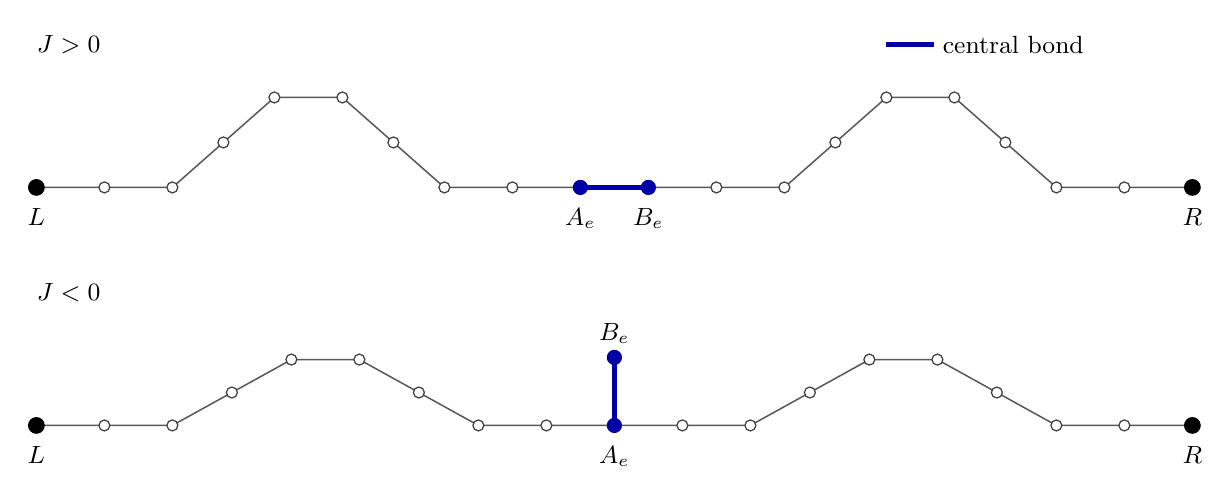
\begin{tikzpicture}[
    x=0.34in,y=0.34in,
    path edge/.style={draw=black!65,line width=0.55pt},
    central edge/.style={draw=blue!65!black,line width=1.6pt},
    site/.style={circle,draw=black!75,fill=white,
      line width=0.45pt,inner sep=1.4pt},
    endpoint/.style={circle,draw=black,fill=black,inner sep=2pt},
    central site/.style={circle,draw=blue!65!black,
      fill=blue!65!black,inner sep=1.8pt},
    every node/.style={font=\small}
  ]
    \pgfmathsetmacro{\positiveHeight}{sqrt(7)/4}
    \pgfmathsetmacro{\positivePeak}{sqrt(7)/2}
    \pgfmathsetmacro{\negativeHeight}{sqrt(15)/8}
    \pgfmathsetmacro{\negativePeak}{sqrt(15)/4}

    \node[anchor=west,inner sep=0pt] at (0,2.1) {$J>0$};
    \draw[central edge] (12.5,2.1) -- (13.2,2.1);
    \node[anchor=west,inner sep=3pt] at (13.2,2.1)
      {central bond};

    \foreach \start in {0,9} {
      \begin{scope}[shift={(\start,0)}]
        \draw[path edge]
          (0,0) -- (1,0) -- (2,0)
          -- (2.75,\positiveHeight) -- (3.5,\positivePeak)
          -- (4.5,\positivePeak) -- (5.25,\positiveHeight)
          -- (6,0) -- (7,0) -- (8,0);
        \foreach \x/\y in {
          0/0,1/0,2/0,2.75/\positiveHeight,3.5/\positivePeak,
          4.5/\positivePeak,5.25/\positiveHeight,6/0,7/0,8/0
        } {
          \node[site] at (\x,\y) {};
        }
      \end{scope}
    }
    \draw[central edge] (8,0) -- (9,0);
    \node[endpoint] at (0,0) {};
    \node[endpoint] at (17,0) {};
    \node[central site] at (8,0) {};
    \node[central site] at (9,0) {};
    \node[anchor=north,inner sep=0pt] at (0,-0.3) {$L$};
    \node[anchor=north,inner sep=0pt] at (8,-0.3) {$A_e$};
    \node[anchor=north,inner sep=0pt] at (9,-0.3) {$B_e$};
    \node[anchor=north,inner sep=0pt] at (17,-0.3) {$R$};

    \begin{scope}[shift={(0,-3.5)}]
      \node[anchor=west,inner sep=0pt] at (0,1.95) {$J<0$};
      \foreach \start in {0,8.5} {
        \begin{scope}[shift={(\start,0)}]
          \draw[path edge]
            (0,0) -- (1,0) -- (2,0)
            -- (2.875,\negativeHeight) -- (3.75,\negativePeak)
            -- (4.75,\negativePeak) -- (5.625,\negativeHeight)
            -- (6.5,0) -- (7.5,0) -- (8.5,0);
          \foreach \x/\y in {
            0/0,1/0,2/0,2.875/\negativeHeight,3.75/\negativePeak,
            4.75/\negativePeak,5.625/\negativeHeight,6.5/0,7.5/0,8.5/0
          } {
            \node[site] at (\x,\y) {};
          }
        \end{scope}
      }
      \draw[central edge] (8.5,0) -- (8.5,1);
      \node[endpoint] at (0,0) {};
      \node[endpoint] at (17,0) {};
      \node[central site] at (8.5,0) {};
      \node[central site] at (8.5,1) {};
      \node[anchor=north,inner sep=0pt] at (0,-0.3) {$L$};
      \node[anchor=north,inner sep=0pt] at (8.5,-0.3) {$A_e$};
      \node[anchor=south,inner sep=0pt] at (8.5,1.2) {$B_e$};
      \node[anchor=north,inner sep=0pt] at (17,-0.3) {$R$};
    \end{scope}
  \end{tikzpicture}
  \caption{The two fixed contact templates, drawn at their actual relative
    coordinates. Every drawn link has length one, and each bent path has
    nine links. The original vertices remain at $L=(0,0)$ and $R=(17,0)$.
    For $J>0$, the central pair is $A_e=(8,0)$, $B_e=(9,0)$ and the paths
    join $L$ to $A_e$ and $B_e$ to $R$. For $J<0$, it is
    $A_e=(8.5,0)$, $B_e=(8.5,1)$ and both paths meet $A_e$.
    Nonlinks are not drawn.}
  \label{fig:contact-templates}
\end{figure}
